\chapter{Placement}
The algorithm for the placement, a determnistic analog circuit placement algorithm using hierarchically bounded enumeration and enhanced shape functions \cite{iccad:plantage}, was developed and implemented mainly by Martin Strasser during his doctoral thesis and by Michael Eick during his diploma thesis. The main idea behind it is, that circuits typically have a certain hierarchy. For example an operation amplifier \nref{fig:miller_amplifier_schematic} consists of a differential amplifier, a current mirror and an output amplifier. Usually it is a good idea to place the modules of the same group not that far away, because they belong together in the logic behind the circuit. This is also the typical way a designer creates a layout out of a circuit manually, he starts with a certain functionality and places the modules for this function together. If the modules are grouped together in the layout \nref{fig:miller_amplifier_layout} they do not see that large differences in for example the temperature of the substrate, which will result in a better performance of the circuit.
At the moment this information about the groups must be fed in by the user, but the target for the future would be, that even this step can be automized by for example a circuit analysis. This information can then be used to find the best placements for these groups, which are then combined on the next level in the hierarchy.

\begin{figure}
	\centering
	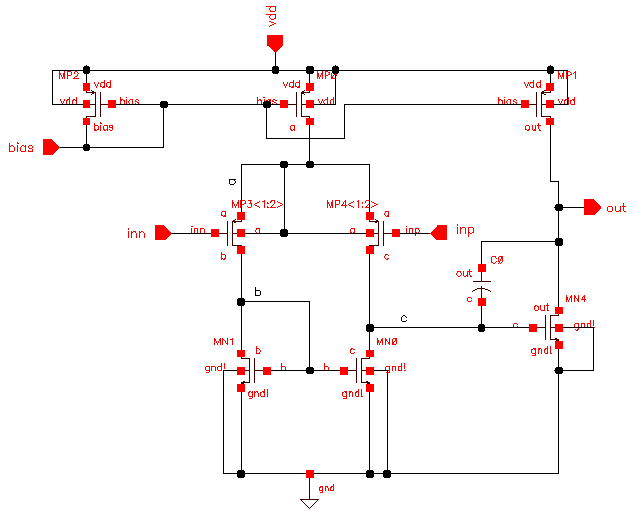
\includegraphics[scale=0.6]{FIG/miller_amplifier_schematic.png}
	\caption{schematic of a miller amplifier}
	\label{fig:miller_amplifier_schematic}
\end{figure}

\begin{figure}
	\centering
	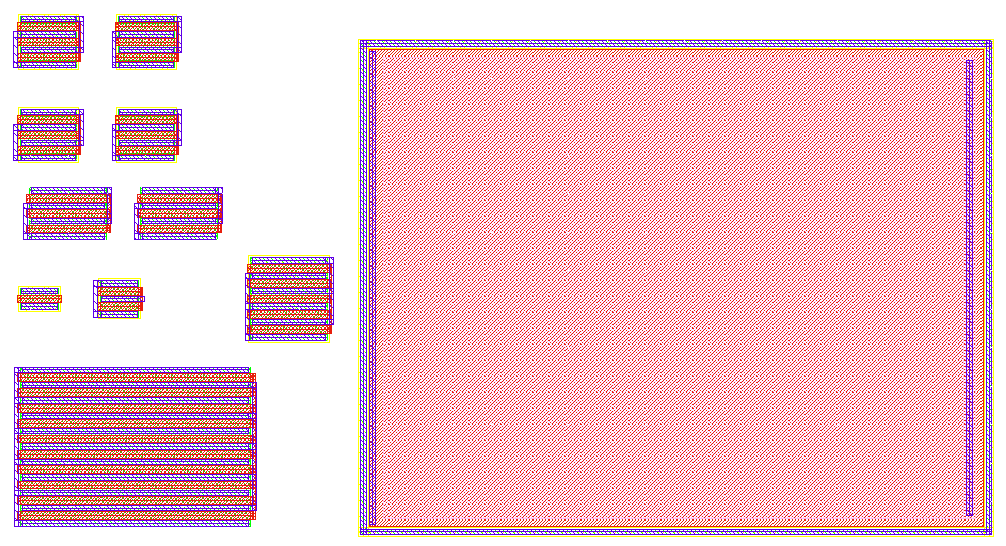
\includegraphics[scale=0.4]{FIG/miller_amplifier_layout.png}
	\caption{possible layout for a miller amplifier}
	\label{fig:miller_amplifier_layout}
\end{figure}

Additionally it is possible to define certain constraints for modules and groups of modules:
\begin{itemize}
\item symmetry
\item alignment
\item group symmetry
\item group alignment
\item same variants
\end{itemize}

Some of these will be later have to be considered by the routing, because for example symmetric modules typically should also have symmetric routes to avoid different resistances of the routes. Furthermore, if we go more in detail, symmetric routes should even have similar capacitive couplings with other routes.

The general structure of this application is divided into two parts:
\begin{itemize}
\item ICFBInterface
\item Plantage
\end{itemize}

First we will start with a short description of Plantage. It is a simple command line tool which accepts an xml input file and produces an xml output file. The input file contains the basic information about the circuit, e.g. the modules with their various variants, group definitions, constraints, and so on. The output file of this tool contains a so called shape funtion with different shapes. The shapes are the actual placements which contain the positions of the modules and the selected variants.

The ICFBInterface is, as its name already tells, an interface between cadence and plantage. It can receive for example the data of a circuit and then guides the user through the process of defining groups and constraints. After this Plantage is executed and the results are displayed. It can even generate real layouts from a selected placement, which was calculated by Plantage.

\section{Algorithm}
As already mentioned before the placement is generated hierarchically. The starting point for the calculation of a placement is an enumeration sequence. This value is a very compact way to store the information of related positions for a bunch of modules. It consists out of a list of boolean variables, usually stored as a string with the values \textit{E} for east and \textit{N} for north. The modules and selected variants for this enumeration are then stored in a B*-tree. On this data structure then the actual calculation of the coordinates, considering the given constraints, is done. From the B*-tree a bunch of lines for a linear program is created. After this linear program is solved by an external application, at the moment lp\textunderscore solve \cite{lp_solve}, the actual coordinates for the modules can be calculated from the solution of the linear program. This is done usually for some different enumerations. The list of possible placements, which is generated that way, is then filtered by the area and only a certain number of placements is then used on the next higher hierarchy level.

\section{Software Architecture}
In the following part the software architecture of only Plantage will be described, as this was the main part for the implementation of the routing. On the side of the GUI only some additional information needed to be displayed or manipulated by the user.

Plantage is a typical example for a grown code base. It contained a lot of different coding styles, had some half implemented features and a lot of old and dead development branches, which were part of the production code. So my first task was to clean this mess up. The main problem here was, that the existing and working features shouldn't be broken, what could had happend easily. For the beginning I generated some test input which covered the most important features. After every risky change I could generate the output from this data and compared it with the results before the changes. Through this practise I was able to slowly refactor the code and increase the encapsulation for some parts. This enabled me to write unit tests for these parts and reduce the risk for broken features even more. One by one I applied this to nearly the complete code base. The result of this is a now well tested and documented code base which easiliy can be changed and improved. Additionally the basic structure of the architecture improved, or better said: An architecture was developed and applied to the code. Therefore it became easier to understand what the different parts of the code actually do. This was also important for the implementation of a routing algorithm, as it by the way produced a single point, where the routing can be done.